Kelompok : 4
Kelas : D4 TI 1A
Anggota : 
1. Damara Benedikta		1174012
2. Duvan Silalahi 		1174011
3. Ilham Habibi			1174028
4. Muhammad Fahmi		1174021
5. Oniwaldus Bere mali	1174005

\section {Frekuensi Serial}
Sebelum kita mengetahui apakah itu frekuensi serial, kita harus tau apakah defenisi dari frekuensi.
\subsection  {defenisi frekuensi}
Frekuensi adalah ukuran jumlah putaran ulang per peristiwa dalam satuan detik dengan satuan Hz.
Untuk menghitung frekuensi, seseorang menetapkan jarak waktu, menghitung jumlah kejadian peristiwa, dan membagi hitungan ini dengan panjang jarak waktu. Pada Sistem Satuan Internasional, hasil perhitungan ini dinyatakan dalam satuan hertz (Hz) yaitu nama pakar fisika Jerman Heinrich Rudolf Hertz yang menemukan fenomena ini pertama kali. Frekuensi sebesar 1 Hz menyatakan peristiwa yang terjadi satu kali per detik.
\section {Frekuensi Serial}
Pada frekuensi serial, setiap saat hanya dibutuhkan 1 bit data yang akan dikirim. Dengan kata lain, bit data akan dikirim satu per satu. frekuensi ini memiliki keuntungan yang hanya membutuhkan satu jalur dan beberapa kabel dibandingkan dengan komunikasi paralel. Pada prinsipnya frekuensi serial adalah frekuensi di mana transmisi data dilakukan per bit sehingga lebih lambat daripada frekuensi paralel, atau dengan kata lain frekuensi serial adalah salah satu metode komunikasi data dimana hanya satu bit data yang dikirimkan melalui seutas kabel pada waktu tertentu.
<<<<<<< HEAD
\section {Frekuensi serial adalah frekuensi yang pengiriman datanya per-bit secara berurutan dan bergantian. Frekuensi ini mempunyai suatu kelebihan yaitu hanya membutuhkan satu jalur dan kabel yang sedikit dibandingkan dengan komunikasi paralel. Pada prinsipnya komunikasi serial merupakanfrekuensi dimana pengiriman data dilakukan per bit sehingga lebih lambat dibandingkan frekuensi parallel, atau dengan kata lain komunikasi serial merupakan salah satu metode komunikasi data di mana hanya satu bit data yang dikirimkan melalui seuntai kabel pada suatu waktu tertentu. Pada dasarnya komunikasi serial adalah kasus khusus komunikasi paralel dengan nilai n = 1, atau dengan kata lain adalah suatu bentuk komunikasi paralel dengan jumlah kabel hanya satu dan hanya mengirimkan satu bit data secara simultan.
\subsection {Hal ini dapat disandingkan dengan komunikasi paralel yang sesungguhnya di mana n-bit data dikirimkan bersamaan, dengan nilai umumnya 8 ≤ n ≤ 128.
=======
<<<<<<< HEAD

\section {ada 2 jenis}
Komunikasi serial terdiri dari dua jenis, serial serial dan sinkron asynchronous. Serial sinkron adalah komunikasi di mana hanya ada satu pihak (pengirim atau penerima) yang menghasilkan jam dan mengirim jam bersama dengan data. Contoh penggunaan serial sinkron ada pada transmisi data keyboard. Asynchronous serial adalah komunikasi di mana kedua pihak (pengirim dan penerima) masing-masing menghasilkan clock tetapi hanya data yang ditransmisikan, tanpa jam. Agar data yang akan ditransmisikan menjadi sama dengan data yang diterima, kedua frekuensi clock harus sama dan harus disinkronkan. Setelah sinkronisasi, pengirim akan mengirim data sesuai dengan frekuensi jam pengirim dan penerima akan membaca data sesuai dengan frekuensi jam penerima. Contoh penggunaan serial asynchronous adalah pada Universal Asynchronous Receiver Transmitter (UART) yang digunakan pada komputer port serial (COM)

=======
\section {serial mode}
Mode serial memerlukan sinkronisasi atau penyesuaian yang berfungsi untuk:
\subsection {fungsi sinkronisasi}
Mengetahui kapan sinyal yang diterimanya adalah sedikit data (bit sinkronisasi)
Mengetahui kapan sinyal yang diterimanya membentuk karakter (sinkronisasi karakter)
Mengetahui kapan sinyal yang diterimanya membentuk blok data (memblokir sinkronisasi)
Selanjutnya, transmisi serial dapat mengambil bentuk dua jenis, yaitu transmisi serial sinkron (sinkron) dan transmisi serial asynchronous (asynchronous). Berikut ini adalah penjelasan dari masing-masing jenis transmisi serial. 
\section Transmisi Serial Sinkron, pengirim akan mengirimkan datanya sesuai dengan frekuensi clock pengirim dan penerima akan membaca data sesuai dengan frekuensi clock penerima. Contoh penggunaan asynchronous serial adalah pada Universal Asynchronous Receiver Transmitter (UART) yang digunakan pada serial port (COM) komputer.
\subsection Antarmuka Kanal serial lebih kompleks/sulit dibandingkan dengan antarmuka melalui
kanal paralel, hal ini disebabkan karena:
\section 1. Dari Segi perangkat keras: adanya proses konversi data pararel menjadi serial atau sebaliknya menggunakan piranti tambahan yang disebut UART (Universal Asynchronous Receiver/Transmitte) dan
2. Dari Segi perangkat lunak: lebih banyak register yang digunakan atau terlibat
\subsection Namun di sisi lain antarmuka kanal serial menawarkan berapa kelebihan dibandingkan secara paralel, antara lain:

>>>>>>> da5ec7e8faaa61dff7bd70ec0b7ddb225ceb48f7
>>>>>>> 546699ff1b4072148b1d901996329551145c5c85

1. Dari Segi perangkat keras: adanya proses konversi data pararel menjadi serial atau sebaliknya menggunakan piranti tambahan yang disebut UART (Universal Asynchronous Receiver/Transmitte) dan
2. Dari Segi perangkat lunak: lebih banyak register yang digunakan atau terlibat
Namun di sisi lain antarmuka kanal serial menawarkan berapa kelebihan dibandingkan secara paralel, antara lain:


1. Kabel untuk komunikasi serial bisa lebih panjang dibandingkan dengan paralel; data-data dalam komunikasi serial dikirim-kan untuk logika ‘1’ sebagai tegangan -3 s/d -25 volt dan untuk logika ‘0’ sebagai tegangan +3 s/d +25 volt, dengan demikian tegangan dalam komunikasi serial memiliki ayunan tegangan maksimum 50 volt, sedangkan pada komunikasi paralel hanya 5 volt. Hal ini menyebabkan gangguan pada kabel-kabel panjang lebih mudah diatasi dibandingkan pada parallel.
15:35 ONI Banyak mikrokontroler yang Namun pada masing-masing komputer dengan komunikasi serial harus dibayar “biaya” antarmuka serial yang agak lebih mahal.
2. Jumlah kabel serial lebih sedikit; Anda bisa menghubungkan dua perangkat komputer yang berjauhan dengan hanya 3 kabel untuk konfigurasi null modem, yaitu TXD (saluran kirim), RXD(saluran terima) dan Ground, bayangkan jika digunakan teknik paralel akan terdapat 20 – 25 kabel. Namun pada masing-masing komputer dengan komunikasi serial harus dibayar “biaya” antarmuka serial yang agak lebih mahal.

3. Banyaknya piranti saat ini (palmtop, organizer, hand-phone dan lainlain) menggunakan teknologi infra merah untuk komunikasi data, dalam hal ini pengiriman datanya dilakukan secara serial. IrDA-1 (spesifikasi infra merah pertama) mampu mengirimkan data dengan laju 115,2 kbps
15:35 ONI dan Konsep Komunikasi Serial 2 dibantu dengan piranti UART, hanya panjang pulsa berkurang menjadi 3/16 dari standar RS-232 untuk menghemat daya.









\section {Pengertian Port}
PENGERTIAN  PORT
Port merupakan satu set perintah yang digunakan oleh komputer untuk memindahkan data dari atau ke perangkat lain, misalnya untuk berhubungan dengan keyboard, mouse, printer, modem, monitor dan sebagainya. Ada berbagai macam port, yaitu :
·         Serial Port
·         Pararel Port
·         IDE
·         SATA
·         USB
·         Ethernet
·         Audio Codec
·         PCI

\section {SERIAL PORT }

	\begin{figure}[ht]
	\centerline{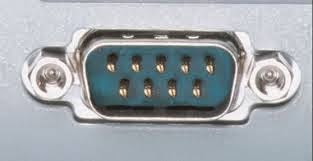
\includegraphics[width=1\textwidth]{figures/port1.jpg}}
	\caption{Implementasi pemetaan memori system paging.}
	\label{Gambar1}
	\end{figure}

	\begin{figure}[ht]
	\centerline{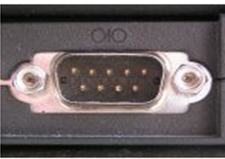
\includegraphics[width=1\textwidth]{figures/port2.jpg}}
	\caption{Implementasi pemetaan memori system paging.}
	\label{Gambar2}
	\end{figure}

\subsection {Pengertian dan Fungsi Serial Port}\ref{Gambar1}
Serial Port atau biasa disebut dalam bahasa Indonesia adalah port seri merupakan sebuah port pada personal computer yang berfungsi untuk mentransmisikan satu bit informasi pada satu satuan waktu. Dalam serial port, pengiriman informasi tidak memungkinkan untuk melakukan secara banyak sekalius. Hal ini disebabkan karena dalam melakukan pemindahan data, biasanya serial port bekerja seri, misalnya COM 1 dan COM 2. Untuk penggunaan port serial sekarang ini sudah berkurang. Penggunaan port serial telah tergantikan dengan port USB dan Firewire. Sedangkan untuk jaringan (networking) fungsinya sudah tergantikan dengan port Ethernet. Berikut beberapa fungsi serial port yaitu menghubungkan antara peripheral (alat) computer lain dengan motherboard, penghubung antara mouse dengan motherboard, penghubung antara modem dengan motherboard, dan mentransmisikan informasi-informasi berupa bit-bit dari mainboard ke perangkat lainnya. Konektor yang digunakan adalah RS-232C dengan 9 pin atau 25 pin. \ref{Gambar2}.

\section {dasar-dasar komunikasi serial}
Saat di mana komputer berkomunikasi dengan dunia luar, semua dilakukan dengan data berukuran byte. Dan hal yang sama, seperti printer, informasi data langsung dilakukan melalui data BUS 8-bit ke 8-bit BUS dari data printer. Ini dapat bekerja selama jaraknya tidak terlalu jauh, mengingat jarak kabel yang panjang akan mengurangi (mengganggu) kualitas sinyal. Kabel yang buruk dan sangat panjang akan membuat logika palsu, dan data menjadi tidak perlu diubah.
<<<<<<< HEAD

\section 
Selain itu, hubungan data 8-bit menjadi sangat mahal, karena dibutuhkan kualitas kabel yang sangat baik dan jumlah yang lebih banyak. Untuk alasan ini, komunikasi serial digunakan untuk mentransfer data antara dua sistem dengan jarak yang sangat jauh mulai dari beberapa puluh meter hingga ribuan kilometer. Gambar 10-1 menunjukkan grafik transfer data serial dan paralel.

\subsection { dasar komunikasi serial }
a. Komunikasi Half- dan Full-Duplex
b. Komunikasi serial Asynchronous dan Data Framing

=======
\subsection {framing data}
Framing data adalah bagaimana suatu rangkaian bit disusun untuk dikirim melalui suatu sistem komunikasi serial.Data yang dikirim melalui komunikasi serial biasanya adalah 5 sampai 9-bit. Pada Arduino, data berukuran sebesar 8-bit (1-byte).
Start dan Stop bit dikenal sebagai synchronization bit. Start dan Stop bit bisa berukuran 2 atau 3-bit. Sesuai dengan namanya, bit-bit ini akan mengawali dan mengakhiri paket data. Start bit selalu berukuran 1-bit, sedangkan Stop bit bisa 1 atau 2-bit. Jika tidak diperlukan untuk dikonfigurasi, biarkan saja nilai Stop bit sebesar 1-bit.

\section {Generasi Serial Port}
PS/2. PS2 merupakan perkembangan dari port serial. Bentuknya berupa bulatan dengan desain sedemikian rupa sehingga tidak mungkin terbalik atau salah. Komputer dengan processor pentium MMX ke atas biasanya terdapat 2 port PS2, yaitu untuk mouse dan keyboard.
Namun saat ini penggunaan port serial sebagain besar sudah digantikan oleh jenis port baru yang bernama USB. Saat ini USB sudah benar-benar diterima pasar dan menggantikan kepopuleran port serial dan port parallel. Saat ini jika kita butuh serial port jenis RS232 atau paralel port(printer port) di sebuah komputer, maka pada saat membeli komputer kita harus memeriksa terlebih dahulu apakah motherboardnya menyediakan serial port dan paralel port. Sedangkan untuk mencari motherboard dengan USB board bukanlah hal yang sulit, umumnya setiap motherboard saat ini telah dilengkapi dengan 2 hingga 4 buah slot port USB dan dua lagi tambahan port USB di bagian depan casing CPU.
>>>>>>> 1cfae4b86747c1021e2d43703f1c095f5aaaaa60

